% Provenance (never printed): cycle 4 SVT, "La planete Terre": sedimentation,
% from sediment to sedimentary rock, fossilisation, fossils and layers as a
% record of past environments; see sources/book1/PROVENANCE.md. Book 1,
% grade 7, chapter 4.
% Vocabulary guard: first chapter allowed to use "sediment"; the principles of
% relative dating (superposition, fossil succession and the rest) and "unconformity" are
% g7.5's and are not named here; fossils as evidence of evolution are the
% biology books' (one sentence of prose).
\chapter{Sedimenten en fossielen}\label{ch:g7:sediments-and-fossils}

De Grand Canyon, in Arizona (Verenigde Staten), is gemiddeld \qty{1.6}{km}
diep. Zijn wanden bestaan uit lagen \omterm{def:g3:stones-pebbles-sand:rock}{gesteente}, de ene boven op de andere,
rood, bruin, grijs en roomkleurig. In de bovenste laag, de Kaibab-kalksteen,
wijzen de boswachters schelpen aan: de schelpen van brachiopoden, dieren die
op de bodem van een \omterm{def:g2:water-on-earth:ocean}{zee} leefden. Dat \omterm{def:g3:stones-pebbles-sand:rock}{gesteente} is op de bodem van een \omterm{def:g2:water-on-earth:ocean}{oceaan}
ontstaan, en het vormt nu de rand van de canyon, hoog boven de \omterm{def:g2:water-on-earth:ocean}{zee}.
% ledger: nps:grca-depth, nps:grca-fossils, nps:grca-kaibab

\begin{omfigure}
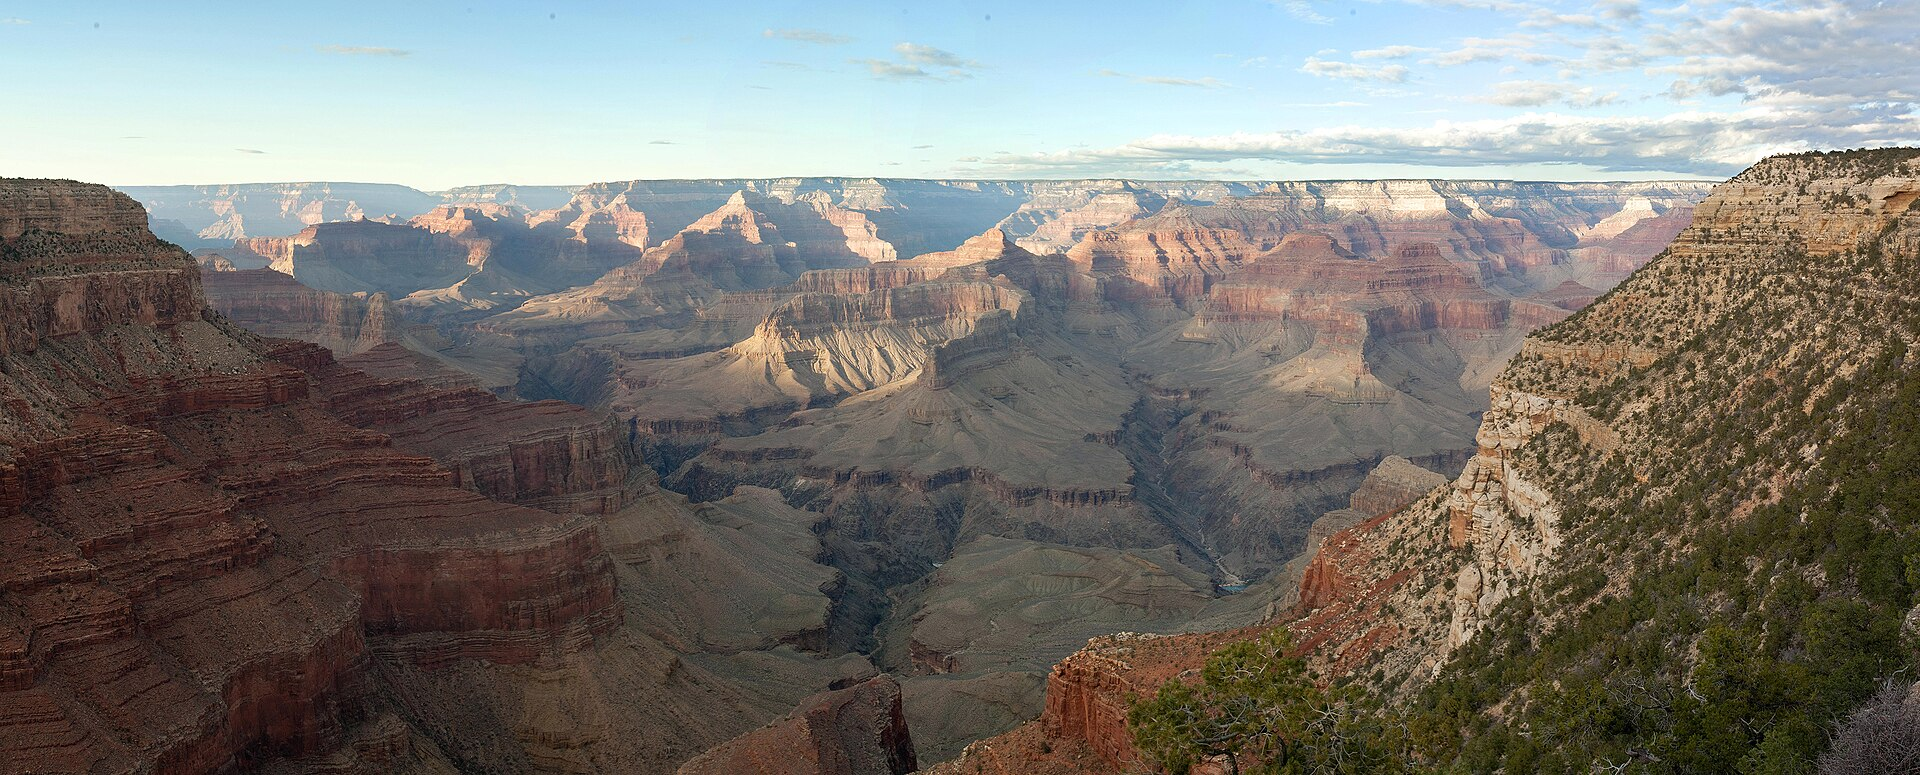
\includegraphics[width=\linewidth]{images/book1/g7-grand-canyon.jpg}

{\small De Grand Canyon vanaf Hermits Rest, op de zuidrand: laag na laag
\omterm{def:g3:stones-pebbles-sand:rock}{gesteente}, van de rand tot op de bodem. Foto van de NPS door Kristen M.
Caldon (publiek domein, via Wikimedia Commons).}
% ledger: commons:grand-canyon
\label{fig:g7:sediments-and-fossils:canyon}
\end{omfigure}

Hoe wordt een hoop los \omterm{def:g3:stones-pebbles-sand:sand}{zand} en modder \omterm{def:g3:stones-pebbles-sand:rock}{vast gesteente}? Hoe kan een schelp zo
lang bewaard blijven dat ze uiteindelijk in een klif terechtkomt? En wat
vertellen lagen en \omterm{def:g7:sediments-and-fossils:fossil}{fossielen} ons over plaatsen zoals ze lang geleden waren?

\begin{recall}
\omterm{def:g3:stones-pebbles-sand:rock}{Gesteente} valt aan het oppervlak langzaam uiteen in stukken
(\emph{\omterm{def:g5:water-shapes-the-land:weathering}{verwering}}); water, wind en ijs voeren de stukken weg
(\emph{\omterm{def:g5:water-shapes-the-land:erosion}{erosie}}) en leggen ze neer waar ze vertragen en stilvallen
(\emph{\omterm{def:g5:water-shapes-the-land:deposition}{afzetting}}): de zwaarste eerst, de fijne modder alleen waar het
water bijna stilstaat (\cref{ch:g5:water-shapes-the-land}). Een
\emph{\omterm{def:g6:rocks-and-minerals:rock-families}{afzettingsgesteente}} ontstaat aan het oppervlak uit korrels \omterm{def:g3:stones-pebbles-sand:sand}{zand} en
modder, of uit schelpen, die in lagen zijn neergelegd en hard zijn
geworden: zandsteen, schalie, kalksteen. De \omterm{def:g6:rocks-and-minerals:rock-cycle}{kringloop van gesteenten}
verandert de \omterm{def:g3:stones-pebbles-sand:rock}{gesteenten} van elke familie langzaam in die van de andere
(\cref{ch:g6:rocks-and-minerals}).
\end{recall}

\section{Sedimenten zetten zich af in lagen}

Overal waar water, wind of ijs laat vallen wat ze meevoerden, groeit een
losse \omterm{def:g5:water-shapes-the-land:deposition}{afzetting} aan: \omterm{def:g3:stones-pebbles-sand:pebble}{grind} en \omterm{def:g3:stones-pebbles-sand:sand}{zand} op een rivierbedding, modder op de bodem
van een \omterm{def:g1:landscapes-around-us:water}{meer}, \omterm{def:g3:stones-pebbles-sand:sand}{zand} op een strand of in een duin, schelpen op de zeebodem.

\begin{definition}[Sediment]\label{def:g7:sediments-and-fossils:sediment}
Een \emph{sediment}\index{sediment} is los materiaal dat door water, wind
of ijs is neergelegd: \omterm{def:g3:stones-pebbles-sand:pebble}{grind}, \omterm{def:g3:stones-pebbles-sand:sand}{zand}, modder, of de schelpen en skeletten van
levende wezens. Het verzamelt zich op de bodem van \omterm{def:g1:landscapes-around-us:water}{rivieren}, \omterm{def:g1:landscapes-around-us:water}{meren} en
\omterm{def:g2:water-on-earth:ocean}{zeeën}, en op het land waar de wind of het ijs het laat vallen.
\end{definition}

\omterm{def:g7:sediments-and-fossils:sediment}{Sedimenten} zetten zich in een bepaalde volgorde af. Als modderig water
vertraagt, zinken de grootste en zwaarste korrels eerst en de kleinste en
lichtste het laatst. Telkens als het water verandert --- een \omterm{def:g5:water-shapes-the-land:flood}{overstroming}
die \omterm{def:g3:stones-pebbles-sand:sand}{zand} aanvoert, daarna rustige weken waarin alleen fijne modder de
bodem bereikt --- veranderen ook de korrels die bezinken, en begint er een
nieuwe laag. Beetje bij beetje raakt de bodem van een \omterm{def:g1:landscapes-around-us:water}{meer} of een \omterm{def:g2:water-on-earth:ocean}{zee}
bedekt met een stapel lagen, met de oudste onderaan.
% ledger: usgs:strata, usgs:sediments-to-rock

\begin{omfigure}
\begin{tikzpicture}[font=\small, x=1cm, y=1cm]
  % land and river
  \fill[omLithAlluv] (0,3.0) -- (2.0,2.45) -- (2.0,0) -- (0,0) -- cycle;
  \fill[blue!35] (0,3.05) -- (2.0,2.5) -- (2.0,2.4) -- (0,2.95) -- cycle;
  % lake water
  \fill[omSea!45] (2.0,2.5) -- (12.4,2.5) -- (12.4,1.12) -- (3.0,1.2) -- cycle;
  \draw[blue!50!black, line width=0.6pt] (2.0,2.5) -- (12.4,2.5);
  % layers on the bottom: thick near the mouth, thinner far out
  \foreach \k/\c in {0/omLithSand, 1/omLithShale, 2/omLithSand, 3/omLithShale} {
    \pgfmathsetmacro{\yb}{0.2+0.25*\k}
    \pgfmathsetmacro{\yt}{0.2+0.25*(\k+1)}
    \fill[\c] (3.0,\yb) -- (12.4,\yb) -- (12.4,\yt-0.08) -- (3.0,\yt) -- cycle;
  }
  \draw[black!60, line width=0.3pt] (3.0,1.2) -- (12.4,1.12);
  \fill[omLithAlluv!80!black] (2.0,0) rectangle (12.4,0.2);
  \fill[omLithAlluv] (2.0,0.2) -- (3.0,0.2) -- (3.0,1.2) -- (2.0,2.45) -- cycle;
  % settling grains: big ones near the mouth, fine ones far out
  \foreach \x/\y in {3.3/2.1, 3.6/1.75, 3.9/2.25, 4.2/1.55, 3.5/1.35, 4.5/2.0} {
    \fill[brown!70!black] (\x,\y) circle (0.07);
    \draw[-{Stealth[length=1.3mm]}, black!60] (\x,\y-0.1) -- (\x,\y-0.32);
  }
  \foreach \x/\y in {6.5/2.2, 7.4/1.8, 8.3/2.15, 9.1/1.6, 9.9/2.05, 10.8/1.75, 11.6/2.1, 7.9/1.35, 10.4/1.3} {
    \fill[brown!50!black] (\x,\y) circle (0.025);
    \draw[-{Stealth[length=1mm]}, black!40] (\x,\y-0.05) -- (\x,\y-0.2);
  }
  \node[anchor=south, align=center] at (1.0,3.1) {de rivier bij hoogwater\\[-2pt]voert zand en\\[-2pt]modder aan};
  \node[anchor=south, align=center] at (4.1,2.55) {het zand bezinkt\\[-2pt]eerst, bij de monding};
  \node[anchor=south, align=center] at (9.2,2.55) {de fijne modder bezinkt langzaam,\\[-2pt]ver weg, waar het water rustig is};
  \draw[decorate, decoration={brace, amplitude=4pt}] (12.55,1.15) -- (12.55,0.2)
    node[midway, anchor=west, xshift=4pt, align=left, font=\footnotesize] {lagen op de\\[-2pt]bodem: zand,\\[-2pt]modder, zand,\\[-2pt]modder};
\end{tikzpicture}

{\small \omterm{def:g7:sediments-and-fossils:sediment}{Sediment} dat bezinkt in een \omterm{def:g1:landscapes-around-us:water}{meer} (een tekening, niet op schaal). Na
elke \omterm{def:g5:water-shapes-the-land:flood}{overstroming} bezinkt een laag \omterm{def:g3:stones-pebbles-sand:sand}{zand}, daarna fijne modder in de rustige
weken die volgen: laag na laag groeit er op de bodem aan.}
% ledger: usgs:strata
\label{fig:g7:sediments-and-fossils:lake}
\end{omfigure}

\begin{definition}[Sedimentlaag]\label{def:g7:sediments-and-fossils:layer}
Een \emph{sedimentlaag}\index{sedimentlaag}, of
\emph{stratum}\index{stratum} (meervoud \emph{strata}), is een plaat
sediment, of het \omterm{def:g3:stones-pebbles-sand:rock}{gesteente} dat eruit is ontstaan, die in één keer is
neergelegd. Ze heeft een basis en een bovenkant, en ze verschilt van de
lagen erboven en eronder in de grootte van haar korrels of in waaruit ze
bestaat.
\end{definition}

\omterm{def:g7:sediments-and-fossils:sediment}{Sedimenten} bezinken uit water of lucht, en worden dus vlak neergelegd,
zoals de bladzijden van een boek dat op een tafel ligt. Als je lagen
scheef of geplooid aantreft, heeft iets ze na hun ontstaan bewogen.
Gelaagdheid is het duidelijkste kenmerk van een \omterm{def:g6:rocks-and-minerals:rock-families}{afzettingsgesteente}: je
zag het in de wanden van de Grand Canyon.
% ledger: usgs:strata, nps:grca-kaibab

\begin{inthelab}[Lagen in een pot (in de klas, met de leraar)]
Doe een handvol \omterm{def:g3:stones-pebbles-sand:pebble}{grind}, twee handen \omterm{def:g3:stones-pebbles-sand:sand}{zand} en een paar lepels aarde in een
hoge glazen pot; vul hem met water, sluit hem goed af en schud hem. Zet hem
neer en kijk een paar minuten: het \omterm{def:g3:stones-pebbles-sand:pebble}{grind} bereikt meteen de bodem, het \omterm{def:g3:stones-pebbles-sand:sand}{zand}
iets later, en de fijne modder houdt het water urenlang troebel. Doe de
volgende dag nog wat aarde en \omterm{def:g3:stones-pebbles-sand:sand}{zand} erbij, schud zachtjes en laat het weer
bezinken. Hoeveel lagen kun je tellen? Welke korrels liggen onderaan elke
laag?
\end{inthelab}

\section{Van sediment tot gesteente}

Een laag blijft niet lang bovenaan. Er bezinken andere lagen bovenop, en
daarna weer andere, en ze komt steeds dieper te liggen. Onder het gewicht
van de lagen erboven worden de korrels dichter tegen elkaar gedrukt en
wordt het water ertussen eruit geperst. Water dat door de stapel sijpelt,
laat tussen de korrels \omterm{def:g6:rocks-and-minerals:mineral}{mineralen} achter, een natuurlijk cement dat ze aan
elkaar kit. Na lange tijd, met nog meer lagen erbovenop en langzame
chemische veranderingen, wordt het losse \omterm{def:g7:sediments-and-fossils:sediment}{sediment} onder in de stapel
\omterm{def:g3:stones-pebbles-sand:rock}{gesteente}.
% ledger: usgs:sediments-to-rock, usgs:sedimentary

Elke soort \omterm{def:g7:sediments-and-fossils:sediment}{sediment} levert zijn eigen \omterm{def:g3:stones-pebbles-sand:rock}{gesteente}.

\begin{center}
\small
\begin{tabular}{|l|l|}
\hline
\textbf{\omterm{def:g7:sediments-and-fossils:sediment}{sediment}} & \textbf{het \omterm{def:g3:stones-pebbles-sand:rock}{gesteente} dat eruit ontstaat} \\
\hline
\omterm{def:g3:stones-pebbles-sand:pebble}{grind} en \omterm{def:g3:stones-pebbles-sand:pebble}{kiezels} & conglomeraat \\
\omterm{def:g3:stones-pebbles-sand:sand}{zand} & zandsteen \\
modder & kleisteen, of schalie als het in dunne platen splijt \\
schelpen en skeletten & kalksteen \\
plantenresten, begraven in een moeras & steenkool \\
\hline
\end{tabular}
\end{center}
% ledger: usgs:sediments-to-rock, usgs:sedimentary, usgs:coal-origin

\begin{omfigure}
\begin{tikzpicture}[font=\small, x=1cm, y=1cm]
  \pgfmathsetseed{11}
  \foreach \p/\gap/\title in {0/0.40/{los sediment}, 1/0.31/{begraven en samengeperst:\\[-2pt]water eruit geperst}, 2/0.31/{verkit: een gesteente}} {
    \begin{scope}[xshift=\p*4.6cm]
      \ifnum\p=2 \fill[black!25] (0,0) rectangle (3.4,3.0);
      \else \fill[omSea!45] (0,0) rectangle (3.4,3.0); \fi
      \foreach \i in {0,...,7} {
        \foreach \j in {0,...,6} {
          \pgfmathsetmacro{\gx}{0.25 + \i*\gap*1.05 + 0.05*rand}
          \pgfmathsetmacro{\gy}{0.25 + \j*\gap + 0.05*rand}
          \pgfmathsetmacro{\gr}{0.13 + 0.03*rand}
          \ifdim\gx pt<3.25pt \ifdim\gy pt<2.85pt
            \fill[omLithSand!80!brown, draw=brown!60!black, line width=0.3pt] (\gx,\gy) circle (\gr);
          \fi\fi
        }
      }
      \draw[black!70, line width=0.6pt] (0,0) rectangle (3.4,3.0);
      \node[anchor=north, align=center] at (1.7,-0.1) {\title};
    \end{scope}
  }
  \draw[-{Stealth[length=2.5mm]}, line width=1pt] (3.6,1.5) -- (4.4,1.5);
  \draw[-{Stealth[length=2.5mm]}, line width=1pt] (8.2,1.5) -- (9.0,1.5);
  \foreach \x in {5.3,6.3,7.3} \draw[-{Stealth[length=2mm]}, line width=0.8pt] (\x,3.7) -- (\x,3.1);
  \node[anchor=south] at (6.3,3.7) {gewicht van de lagen erboven};
  \node[anchor=south, font=\footnotesize, align=center] at (10.9,3.05) {grijs: het natuurlijke cement};
\end{tikzpicture}

{\small Van \omterm{def:g3:stones-pebbles-sand:sand}{zand} tot zandsteen (een tekening van de korrels, sterk
vergroot). Links: losse korrels met water ertussen. Midden: begraven onder
nieuwe lagen worden de korrels tegen elkaar gedrukt. Rechts: \omterm{def:g6:rocks-and-minerals:mineral}{mineralen} die
het water achterlaat, kitten de korrels aan elkaar.}
% ledger: usgs:sediments-to-rock, usgs:sedimentary
\label{fig:g7:sediments-and-fossils:to-rock}
\end{omfigure}

De meeste \omterm{def:g3:stones-pebbles-sand:rock}{gesteenten} die je aan het aardoppervlak ziet, zijn
\omterm{def:g6:rocks-and-minerals:rock-families}{afzettingsgesteenten}. De stapel lagen die ze vormen, is het
geschiedenisboek van de plek: elke laag is een bladzijde, en de oudste
bladzijden liggen onderaan.
% ledger: usgs:sediments-to-rock

\section{Hoe een fossiel ontstaat}

\begin{definition}[Fossiel]\label{def:g7:sediments-and-fossils:fossil}
Een \emph{fossiel}\index{fossiel} is het overblijfsel, of het spoor, van
een levend wezen van lang geleden, bewaard in \omterm{def:g3:stones-pebbles-sand:rock}{gesteente}. Sommige fossielen
zijn de harde delen van het lichaam --- een schelp, een bot, een tand,
hout --- die in steen zijn veranderd. Andere bewaren alleen een vorm: een
\emph{afdruk}\index{afdruk} is de holle indruk die in het \omterm{def:g3:stones-pebbles-sand:rock}{gesteente}
achterblijft waar een schelp of een bot is opgelost; een
\emph{afgietsel}\index{afgietsel} is de kopie die ontstaat als een afdruk
wordt opgevuld met nieuwe minerale stof of \omterm{def:g7:sediments-and-fossils:sediment}{sediment}. Een
\emph{sporenfossiel}\index{sporenfossiel} is een teken van wat een dier
deed --- een voetafdruk, een graafgang, een sleepspoor --- en geen deel van
zijn lichaam.
\end{definition}

Een \omterm{def:g7:sediments-and-fossils:fossil}{fossiel} begint zijn bestaan als een dood dier of een dode plant op de
bodem van een \omterm{def:g2:water-on-earth:ocean}{zee} of een \omterm{def:g1:landscapes-around-us:water}{meer}. Als het onbedekt blijft, breken bacteriën
het af en lost het water langzaam op wat er overblijft. Het maakt alleen
een kans als het snel wordt begraven, onder \omterm{def:g7:sediments-and-fossils:sediment}{sediment} dat erover bezinkt en
het afsluit. Terwijl het \omterm{def:g7:sediments-and-fossils:sediment}{sediment} daarna in \omterm{def:g3:stones-pebbles-sand:rock}{gesteente} verandert, brengt
water dat door de lagen sijpelt \omterm{def:g6:rocks-and-minerals:mineral}{mineralen} mee die elk piepklein gaatje in
de schelp of het bot opvullen: het verandert in steen. Lang daarna kunnen
de lagen erboven wegslijten, en komt het \omterm{def:g7:sediments-and-fossils:fossil}{fossiel} aan het oppervlak.
% ledger: ucmp:fossil-conditions, ucmp:fossil-kinds, usgs:sediments-to-rock

\begin{omfigure}
\begin{tikzpicture}[font=\small, x=0.86cm, y=0.86cm,
    shell/.pic={
      \fill[#1] (0,0) circle (0.42);
      \draw[brown!40!black, line width=0.5pt] plot[domain=0:12.5, samples=90, smooth]
        ({0.032*\x*cos(\x r)}, {0.032*\x*sin(\x r)});
      \draw[brown!40!black, line width=0.5pt] (0,0) circle (0.42);
    }]
  % 1: death on the sea floor
  \begin{scope}[xshift=0cm]
    \fill[omSea!45] (0,1.2) rectangle (3.3,3.6);
    \fill[omLithShale] (0,0) rectangle (3.3,1.2);
    \pic at (1.65,1.62) {shell=omLithSand!60!white};
    \node[anchor=north, align=center] at (1.65,-0.1) {1. het sterft op\\[-2pt]de zeebodem};
  \end{scope}
  % 2: quick burial
  \begin{scope}[xshift=3.75cm]
    \fill[omSea!45] (0,2.1) rectangle (3.3,3.6);
    \fill[omLithShale] (0,0) rectangle (3.3,1.2);
    \fill[omLithShale!70!white] (0,1.2) rectangle (3.3,2.1);
    \pic at (1.65,1.62) {shell=omLithSand!60!white};
    \foreach \x in {0.5,1.2,2.1,2.8} \fill[brown!50!black] (\x,2.4) circle (0.03);
    \node[anchor=north, align=center] at (1.65,-0.1) {2. modder bedekt\\[-2pt]het snel};
  \end{scope}
  % 3: buried deep, turned to stone
  \begin{scope}[xshift=7.5cm]
    \fill[omLithShale!80!black] (0,0) rectangle (3.3,1.2);
    \fill[omLithShale!85!black] (0,1.2) rectangle (3.3,2.1);
    \fill[omLithSand] (0,2.1) rectangle (3.3,2.9);
    \fill[omLithLime] (0,2.9) rectangle (3.3,3.6);
    \pic at (1.65,1.62) {shell=black!35};
    \node[anchor=north, align=center] at (1.65,-0.1) {3. diep begraven\\[-2pt]wordt het steen};
  \end{scope}
  % 4: uncovered by erosion
  \begin{scope}[xshift=11.25cm]
    \fill[white] (0,0) rectangle (3.3,3.6);
    \fill[omLithShale!80!black] (0,0) -- (3.3,0) -- (3.3,2.6) -- (2.4,2.3) -- (1.8,1.95) -- (1.2,1.7) -- (0,1.5) -- cycle;
    \draw[black!35, line width=0.4pt] (0,1.2) -- (3.3,1.2);
    \draw[black!60, line width=0.4pt] (0,1.5) -- (1.2,1.7) -- (1.8,1.95) -- (2.4,2.3) -- (3.3,2.6);
    \pic at (1.65,1.84) {shell=black!35};
    \node[anchor=north, align=center] at (1.65,-0.1) {4. erosie brengt het\\[-2pt]aan het oppervlak};
  \end{scope}
  \foreach \p in {0,1,2,3} {
    \begin{scope}[xshift=\p*3.75cm]
      \draw[black!70, line width=0.5pt] (0,0) rectangle (3.3,3.6);
    \end{scope}
  }
\end{tikzpicture}

{\small Hoe een \omterm{def:g7:sediments-and-fossils:fossil}{fossiel} ontstaat (een tekening, niet op schaal): een schelp
wordt snel onder modder begraven; dieper begraven onder nieuwe lagen
verandert ze in steen; lang daarna slijt de \omterm{def:g5:water-shapes-the-land:erosion}{erosie} de lagen erboven weg en
komt het \omterm{def:g7:sediments-and-fossils:fossil}{fossiel} aan het oppervlak.}
% ledger: ucmp:fossil-conditions, ucmp:fossil-kinds
\label{fig:g7:sediments-and-fossils:steps}
\end{omfigure}

De meeste levende wezens laten helemaal geen \omterm{def:g7:sediments-and-fossils:fossil}{fossiel} achter. Zachte
lichamen rotten weg voordat ze kunnen worden begraven; zelfs schelpen en
botten breken of lossen op als ze lang onbedekt liggen. De beste plek om
een \omterm{def:g7:sediments-and-fossils:fossil}{fossiel} te worden is de bodem van een rustige \omterm{def:g2:water-on-earth:ocean}{zee} of een rustig meer,
waar fijne modder over de resten bezinkt en ze beschermt. Daarom zijn de
\omterm{def:g7:sediments-and-fossils:fossil}{fossielen} die in \omterm{def:g3:stones-pebbles-sand:rock}{gesteenten} worden gevonden vooral schelpen, en de
piepkleine schelpjes en resten van microscopisch kleine planten en dieren;
dinosaurussen, de bekendste \omterm{def:g7:sediments-and-fossils:fossil}{fossielen}, vormen er maar een heel klein deel
van.
% ledger: ucmp:fossil-conditions, usgs:fossil-record-shells

\begin{omfigure}
\begin{minipage}[t]{0.49\linewidth}\centering
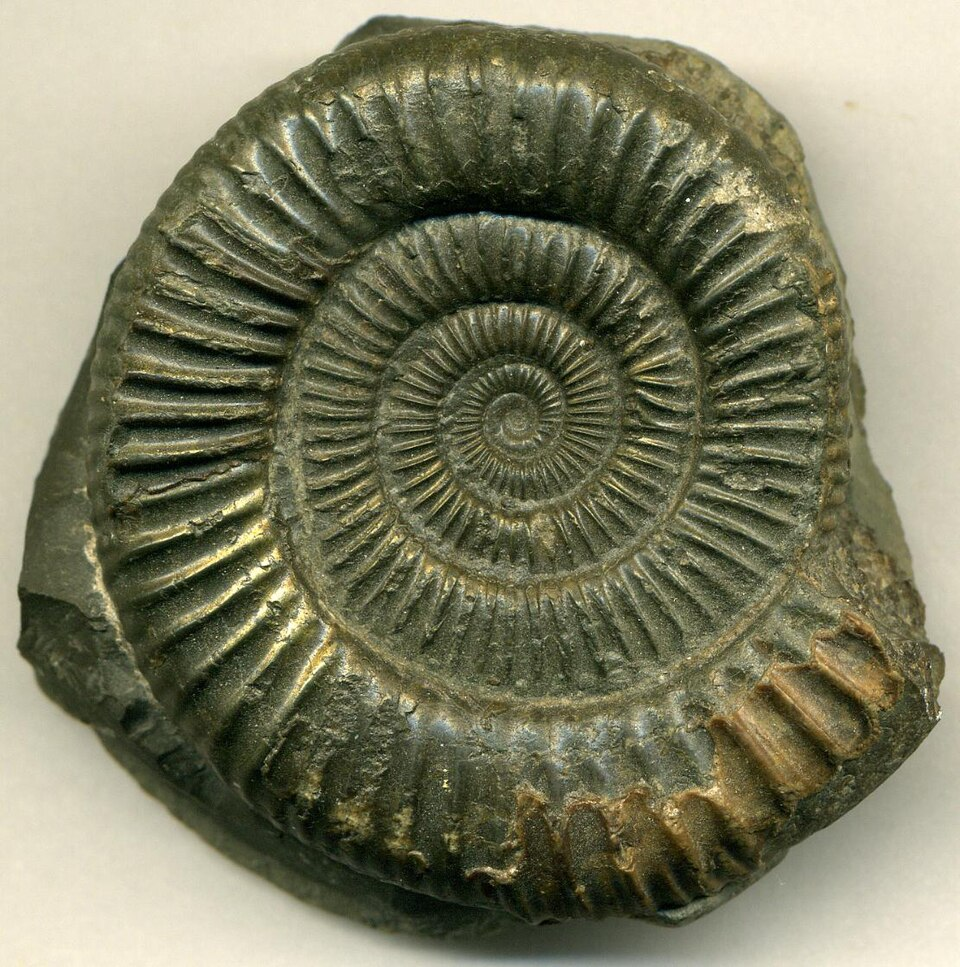
\includegraphics[height=4.6cm]{images/book1/g7-ammonite.jpg}

{\small Een ammoniet, een uitgestorven dier met een opgerolde schelp, een
verwant van de inktvissen en octopussen, \qty{5.7}{cm} in doorsnee, van de
\omterm{def:g1:landscapes-around-us:water}{kust} van Yorkshire (Engeland).}
\end{minipage}\hfill
\begin{minipage}[t]{0.49\linewidth}\centering
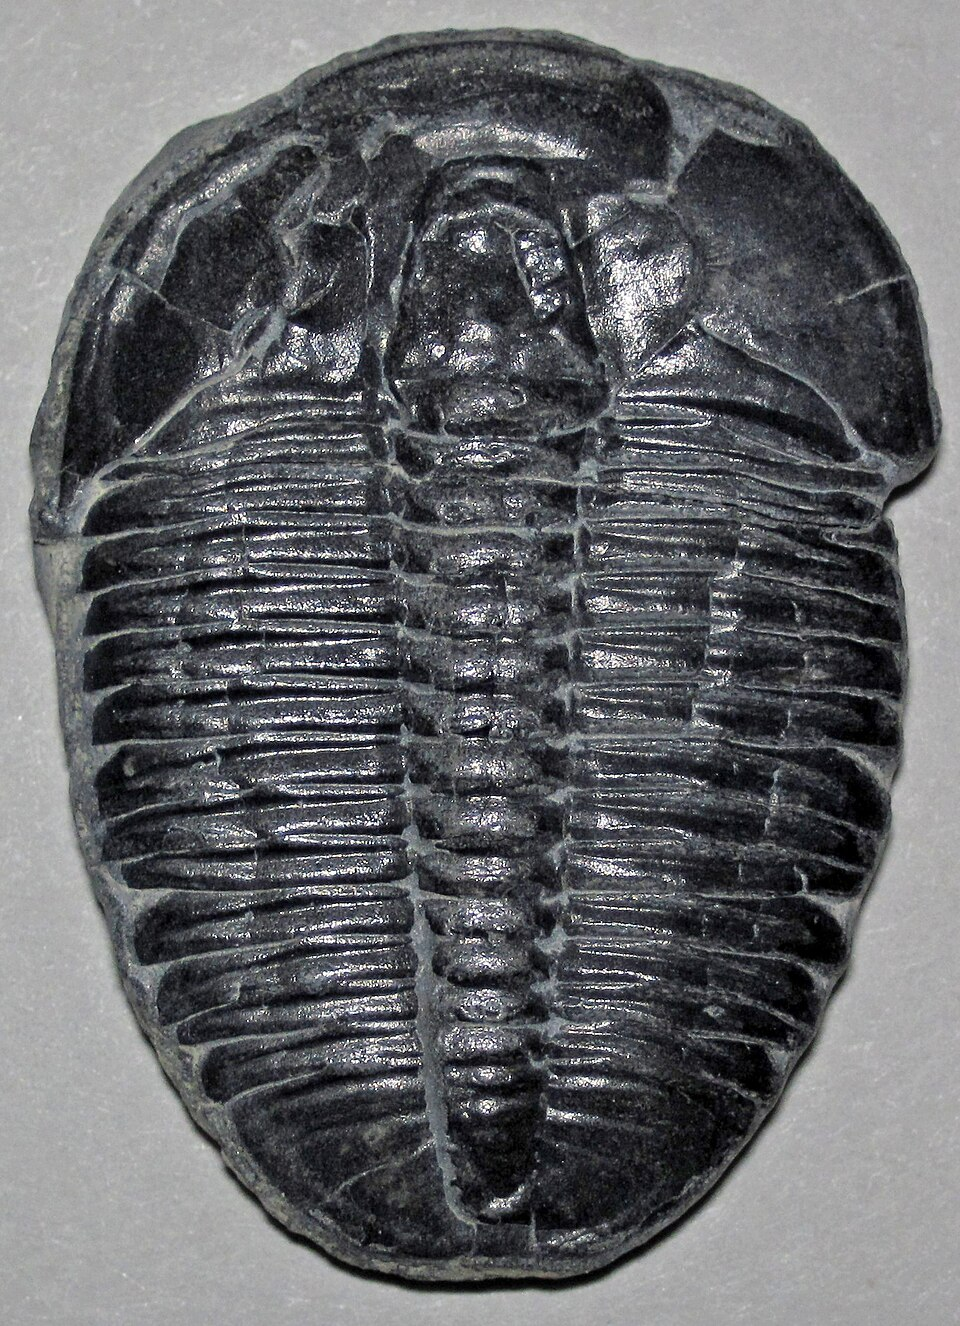
\includegraphics[height=4.6cm]{images/book1/g7-trilobite.jpg}

{\small Een trilobiet, een uitgestorven zeedier waarvan het lichaam uit
drie lobben bestaat, ongeveer \qty{2.6}{cm} breed, uit Utah (Verenigde
Staten).}
\end{minipage}\par\medskip

{\small Twee \omterm{def:g7:sediments-and-fossils:fossil}{fossielen} van dieren met een harde schaal. Foto's: James
St.~John (CC BY 2.0, via Wikimedia Commons).}
% ledger: commons:ammonite, commons:trilobite, nps:ammonoid, nps:trilobite
\label{fig:g7:sediments-and-fossils:ammonite-trilobite}
\end{omfigure}

Soms blijft de schelp zelf niet bewaard. Begraven in \omterm{def:g3:stones-pebbles-sand:sand}{zand} wordt ze langzaam
opgelost door het water dat tussen de korrels door sijpelt, en blijft er
alleen een holte over, met de vorm van de schelp in de wanden gedrukt: een
\omterm{def:g7:sediments-and-fossils:fossil}{afdruk}. Als er later \omterm{def:g6:rocks-and-minerals:mineral}{mineralen} in de holte neerslaan en die opvullen,
vormen ze een kopie van de schelp: een \omterm{def:g7:sediments-and-fossils:fossil}{afgietsel}.
% ledger: ucmp:casts-molds

\begin{omfigure}
\begin{tikzpicture}[font=\small, x=1cm, y=1cm,
    clam/.style={line width=0.5pt}]
  \foreach \p/\fillc/\title in {0/{omLithSand!50!white}/{een schelp begraven\\[-2pt]in zand}, 1/{white}/{de schelp is opgelost:\\[-2pt]een afdruk}, 2/{black!40}/{mineralen vullen de afdruk:\\[-2pt]een afgietsel}} {
    \begin{scope}[xshift=\p*4.9cm]
      \fill[omLithSand] (0,0) rectangle (4.2,2.6);
      \foreach \i in {0,...,40} {
        \pgfmathsetmacro{\gx}{0.1+mod(\i*0.53,4.0)}
        \pgfmathsetmacro{\gy}{0.1+mod(\i*0.37,2.4)}
        \fill[brown!60!black] (\gx,\gy) circle (0.025);
      }
      \fill[\fillc, draw=brown!40!black, clam] (0.9,0.9) arc[start angle=180, end angle=0, x radius=1.2, y radius=0.95] -- cycle;
      \ifnum\p=1
        \foreach \a in {25,45,...,155} \draw[brown!50!black, line width=0.4pt] (2.1,0.9) -- ++(\a:0.93 and 0.75);
      \else
        \foreach \a in {25,45,...,155} \draw[brown!40!black, line width=0.4pt] (2.1,0.9) -- ++(\a:1.05 and 0.85);
      \fi
      \draw[black!70, line width=0.5pt] (0,0) rectangle (4.2,2.6);
      \node[anchor=north, align=center] at (2.1,-0.1) {\title};
    \end{scope}
  }
  \draw[-{Stealth[length=2.5mm]}, line width=1pt] (4.3,1.3) -- (4.8,1.3);
  \draw[-{Stealth[length=2.5mm]}, line width=1pt] (9.2,1.3) -- (9.7,1.3);
\end{tikzpicture}

{\small Een \omterm{def:g7:sediments-and-fossils:fossil}{afdruk} en een \omterm{def:g7:sediments-and-fossils:fossil}{afgietsel} (een tekening, dwars door het
\omterm{def:g3:stones-pebbles-sand:rock}{gesteente}). De \omterm{def:g7:sediments-and-fossils:fossil}{afdruk} is de holte, met de ribbels van de schelp in haar
wand gedrukt; het \omterm{def:g7:sediments-and-fossils:fossil}{afgietsel} is een stenen kopie van de schelp, gemaakt van
de \omterm{def:g6:rocks-and-minerals:mineral}{mineralen} die de holte opvulden.}
% ledger: ucmp:casts-molds
\label{fig:g7:sediments-and-fossils:mould-cast}
\end{omfigure}

Dieren laten ook \omterm{def:g7:sediments-and-fossils:fossil}{fossielen} achter van wat ze deden. Een dier dat over de
zachte, natte modder van een rivieroever of een \omterm{def:g1:landscapes-around-us:water}{kust} loopt, laat
voetafdrukken achter. De meeste worden door de volgende golf of de
volgende \omterm{def:g5:water-shapes-the-land:flood}{overstroming} weggespoeld. Maar als \omterm{def:g3:stones-pebbles-sand:sand}{zand} ze bedekt voordat ze zijn
uitgewist, wordt de voetafdruk opgevuld, wordt het \omterm{def:g3:stones-pebbles-sand:sand}{zand} later zandsteen,
en als het \omterm{def:g3:stones-pebbles-sand:rock}{gesteente} langs de laag splijt, toont het de voetafdruk en, aan
de andere kant, het \omterm{def:g7:sediments-and-fossils:fossil}{afgietsel} ervan.
% ledger: ucmp:footprints

\begin{omfigure}
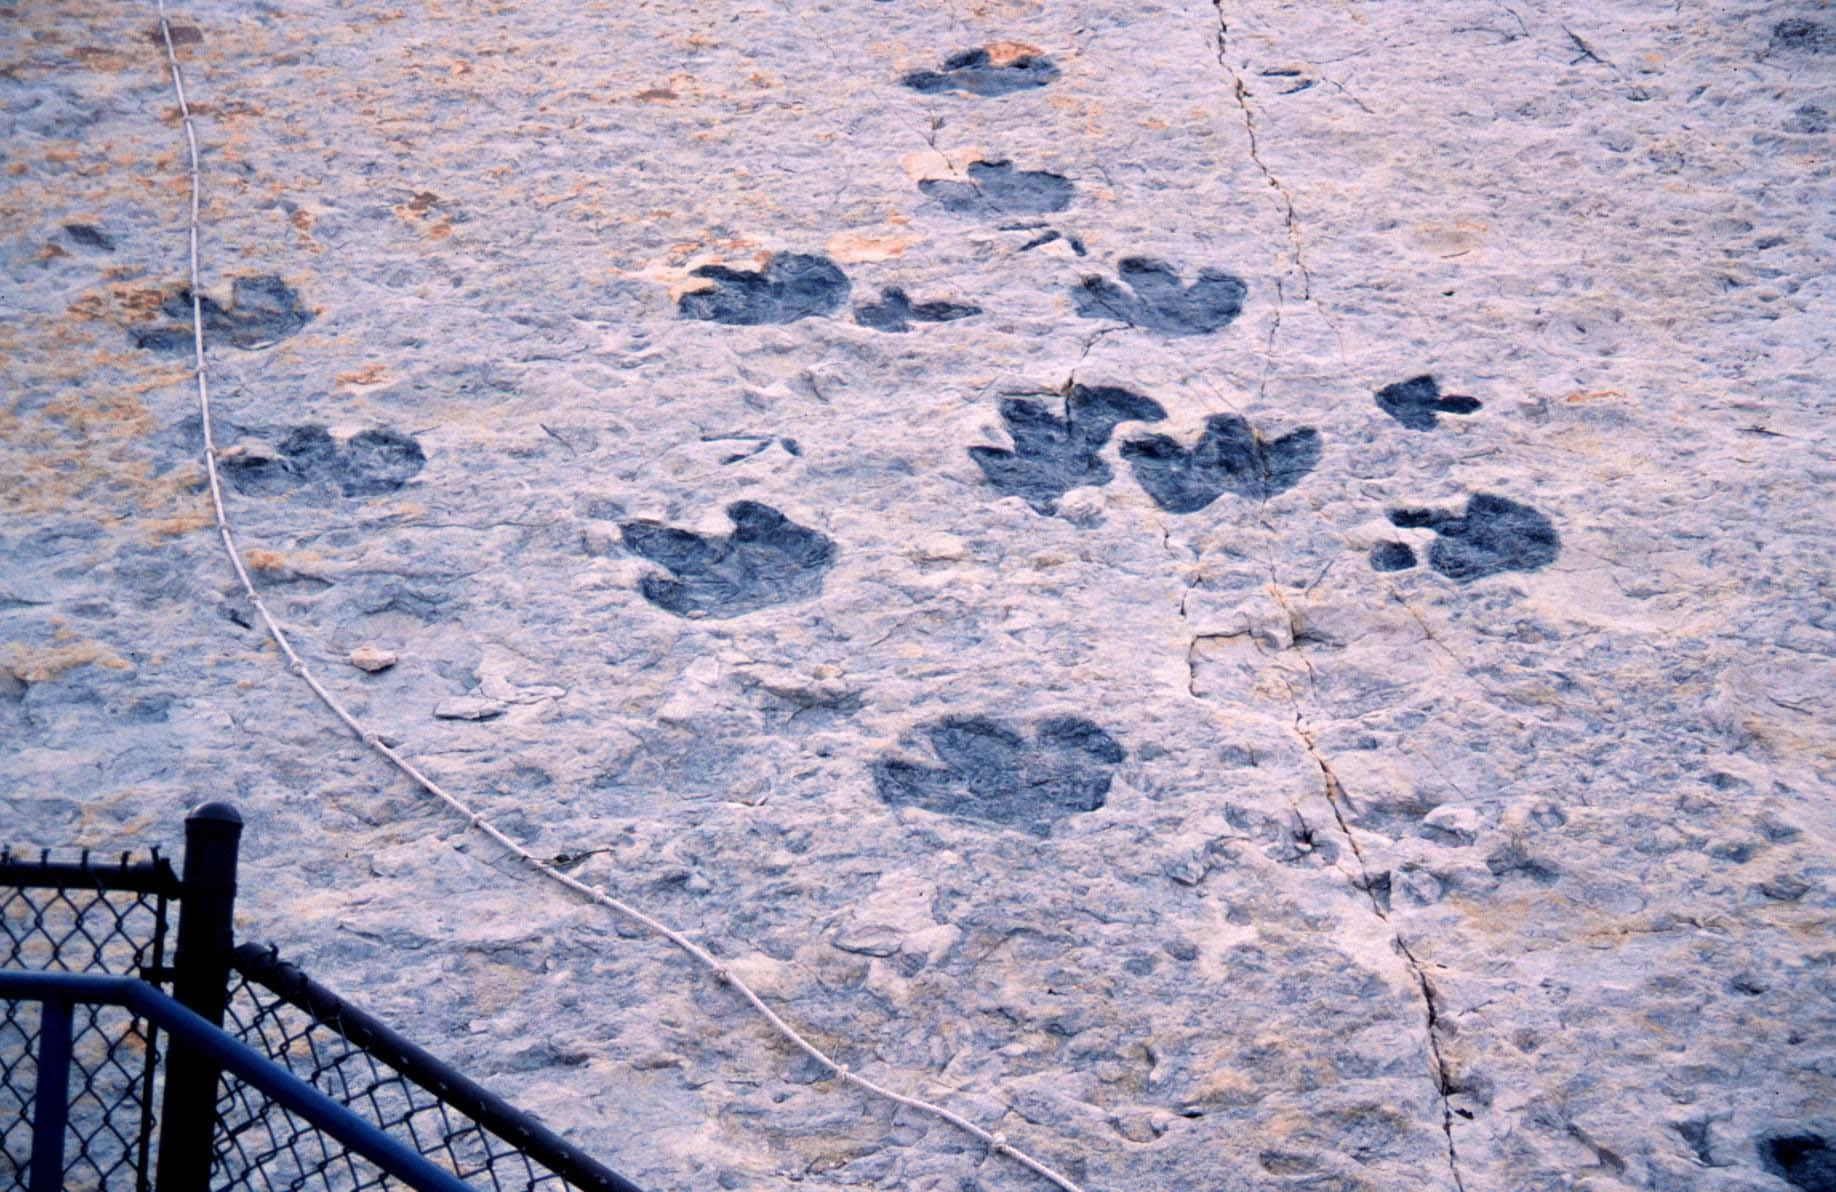
\includegraphics[width=0.62\linewidth]{images/book1/g7-dinosaur-tracks.jpg}

{\small Voetafdrukken van dinosaurussen bij Dinosaur Ridge, bij Morrison,
Colorado (Verenigde Staten): tientallen sporen die in zachte grond zijn
achtergelaten en nu een scheef rotsvlak vormen. De meeste zijn gemaakt door
plantenetende dinosaurussen, een paar door vleeseters met slanke tenen.
Foto: Dexter Perkins (CC0, via Wikimedia Commons).}
% ledger: commons:dino-tracks
\label{fig:g7:sediments-and-fossils:tracks}
\end{omfigure}

De biologie gebruikt \omterm{def:g7:sediments-and-fossils:fossil}{fossielen} om de lange geschiedenis van het leven te
volgen. In dit boek zijn \omterm{def:g7:sediments-and-fossils:fossil}{fossielen} aanwijzingen van een andere soort: ze
vertellen ons hoe de plek eruitzag toen het dier er leefde.

\section{Lagen en fossielen, een archief van het verleden}

Elke laag bewaart de sporen van de plek waar ze werd neergelegd. Koraalriffen
groeien nu in warme, heldere, ondiepe \omterm{def:g2:water-on-earth:ocean}{zeeën}; golfribbels ontstaan in \omterm{def:g3:stones-pebbles-sand:sand}{zand}
in ondiep water, aan de rand van een \omterm{def:g1:landscapes-around-us:water}{meer}, een \omterm{def:g1:landscapes-around-us:water}{rivier} of een \omterm{def:g2:water-on-earth:ocean}{zee}; steenkool
ontstond uit de planten van oude wouden en moerassen; brachiopoden,
zeelelies en trilobieten leefden alleen in de \omterm{def:g2:water-on-earth:ocean}{zee}. Als je dezelfde
aanwijzingen in een oude laag vindt, zag de plek er waarschijnlijk zo uit
toen de laag ontstond.
% ledger: noaa:coral-where, nps:ripple-marks, nps:ripples-shallow, usgs:coal-origin, nps:trilobite

\begin{center}
\small
\begin{tabular}{|p{0.36\linewidth}|p{0.52\linewidth}|}
\hline
\textbf{aanwijzing in de laag} & \textbf{de plek toen de laag ontstond} \\
\hline
koralen & een warme, ondiepe, heldere \omterm{def:g2:water-on-earth:ocean}{zee} \\
\hline
schelpen van zeedieren (brachiopoden, zeelelies, trilobieten) & een \omterm{def:g2:water-on-earth:ocean}{zee} \\
\hline
golfribbels op het oppervlak van een laag & ondiep water, aan de rand van een \omterm{def:g1:landscapes-around-us:water}{meer}, een \omterm{def:g1:landscapes-around-us:water}{rivier} of een \omterm{def:g2:water-on-earth:ocean}{zee} \\
\hline
voetafdrukken & zachte, natte modder of \omterm{def:g3:stones-pebbles-sand:sand}{zand}, vaak aan een \omterm{def:g1:landscapes-around-us:water}{kust} of een rivieroever \\
\hline
steenkool & een moerasbos of een moeras \\
\hline
bladeren en vleugels van libellen & land, met groeiende planten \\
\hline
\end{tabular}
\end{center}
% ledger: noaa:coral-where, nps:grca-fossils, nps:trilobite, nps:ripple-marks, nps:ripples-shallow, ucmp:footprints, usgs:coal-origin

\begin{method}[Een laag lezen]\label{met:g7:sediments-and-fossils:reading}
\begin{enumerate}
  \item Kijk naar de korrels: grove korrels bezinken waar het water snel
        stroomt, fijne modder alleen waar het rustig is.
  \item Zoek naar \omterm{def:g7:sediments-and-fossils:fossil}{fossielen} en sporen (koralen, schelpen, voetafdrukken,
        golfribbels, plantenresten, steenkool) en gebruik de tabel
        hierboven.
  \item Voeg de aanwijzingen samen tot één beeld van de plek: land of \omterm{def:g2:water-on-earth:ocean}{zee},
        ondiep of diep, rustig of stromend water.
\end{enumerate}
\end{method}

\begin{omfigure}
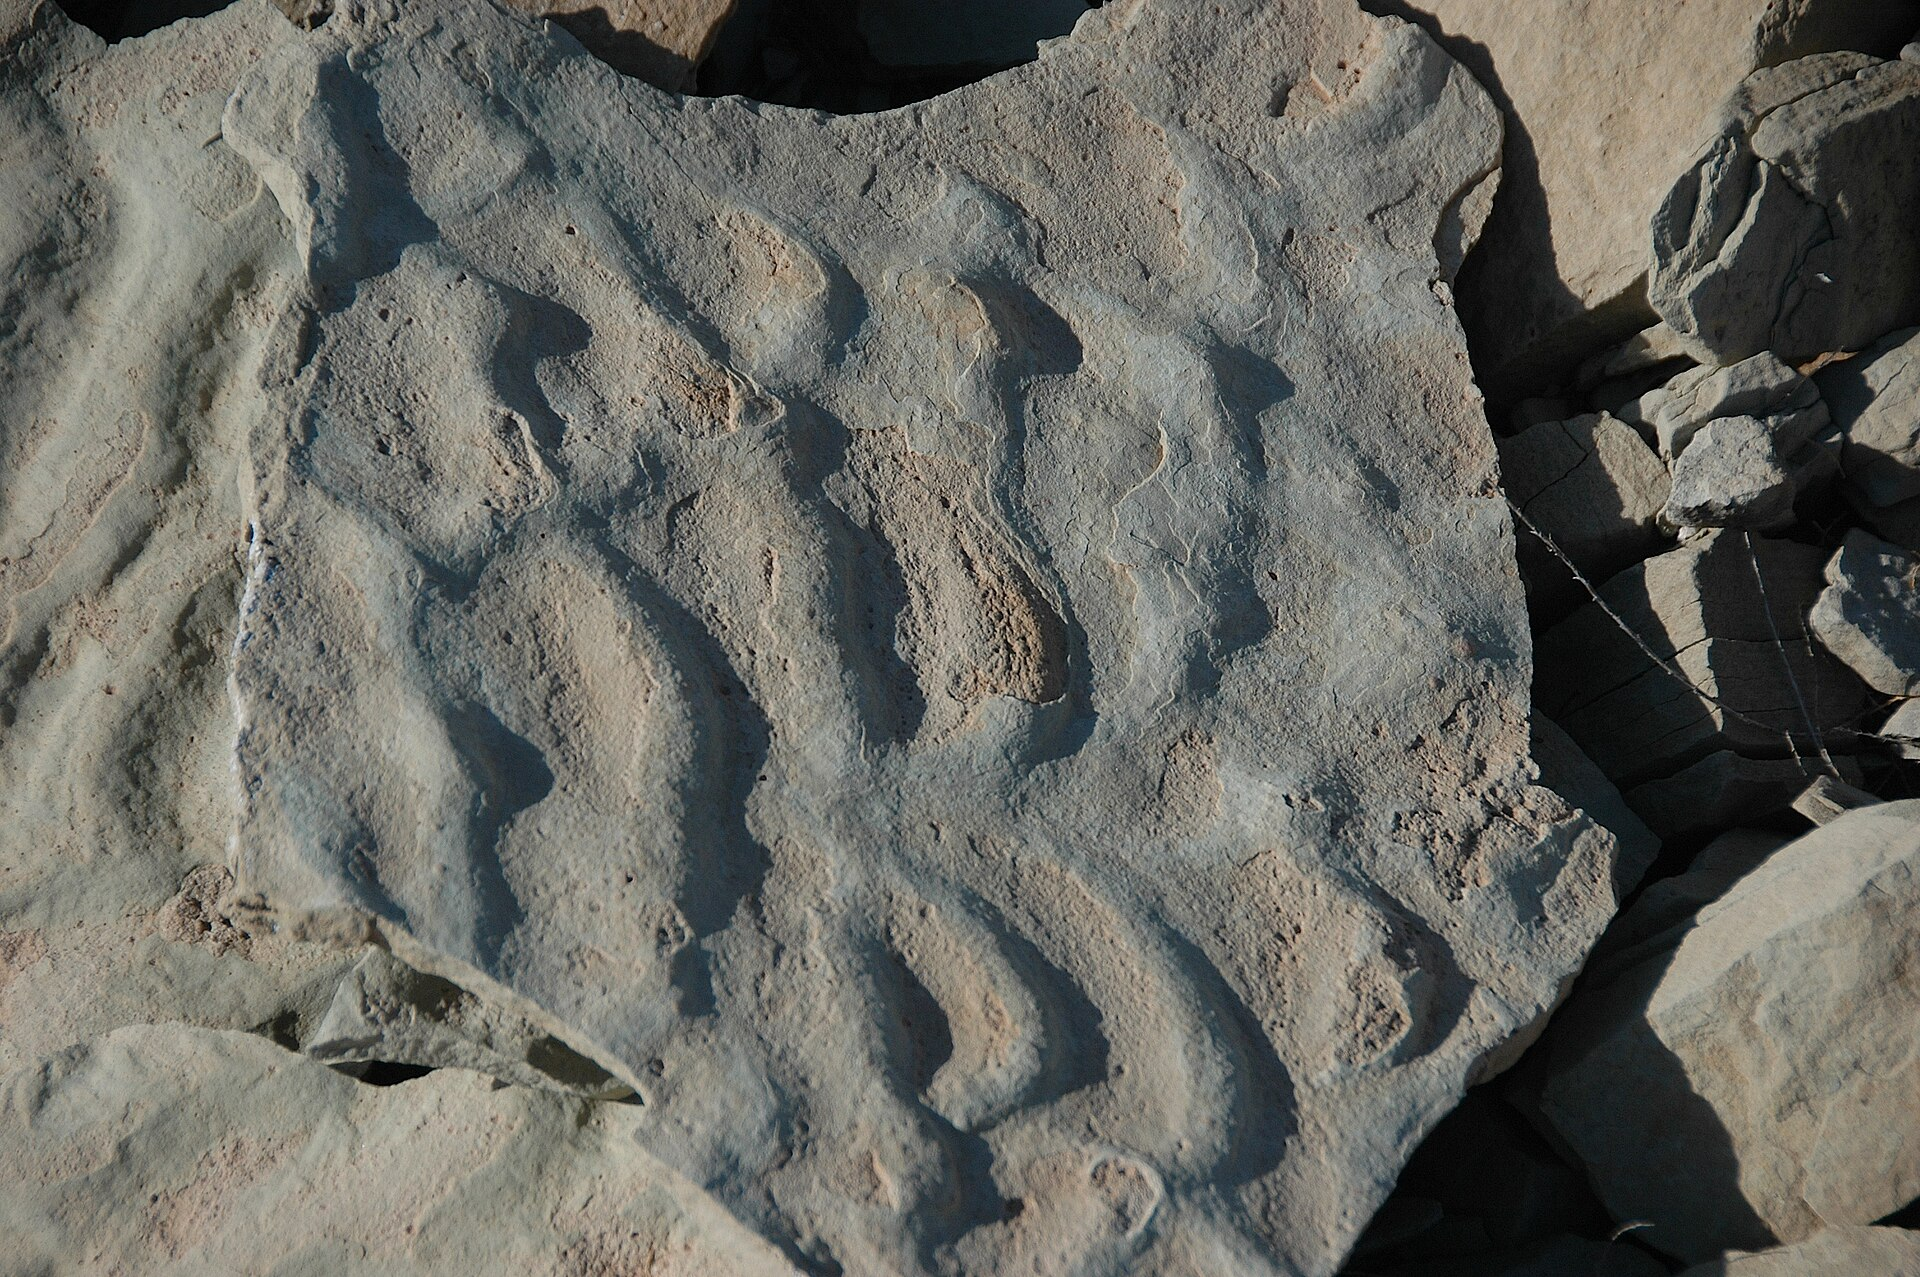
\includegraphics[width=0.56\linewidth]{images/book1/g7-ripple-marks.jpg}

{\small Golfribbels op een plaat zandsteen in Capitol Reef National Park,
Utah (Verenigde Staten): het \omterm{def:g3:stones-pebbles-sand:sand}{zand} werd ooit door stromend water tot ribbels
gevormd, zoals het \omterm{def:g3:stones-pebbles-sand:sand}{zand} van een strand of een beekbedding nu. Foto: James
St.~John (CC BY 2.0, via Wikimedia Commons).}
% ledger: commons:ripples, nps:ripple-marks
\label{fig:g7:sediments-and-fossils:ripples}
\end{omfigure}

\begin{example}[De top van de Grand Canyon]\label{ex:g7:sediments-and-fossils:kaibab}
De Kaibab-kalksteen, de bovenste laag van de Grand Canyon, zit vol schelpen
van brachiopoden en stukjes van de stengels van zeelelies, allebei
zeedieren. Hij is op de bodem van een \omterm{def:g2:water-on-earth:ocean}{zee} ontstaan. Vandaag ligt dezelfde
laag tot ongeveer \qty{2700}{m} (\num{9000}~voet) boven \omterm{def:g4:world-physical-map:altitude}{zeeniveau}: sinds
zijn ontstaan is het hele gebied omhooggekomen.
% ledger: nps:grca-fossils, nps:grca-kaibab
\end{example}

Een stapel lagen kan worden getekend als een \emph{kolom}: de lagen op
elkaar in de volgorde waarin ze ontstonden, met hun dikte op schaal en hun
aanwijzingen ernaast genoteerd. Hieronder staat de kolom van de Varden
Hills, het verzonnen gebied van de oefeningen in deze reeks.

\begin{omfigure}
\begin{tikzpicture}
  \begin{axis}[width=4.2cm, height=9.2cm, scale only axis=false, xmin=0, xmax=1, ymin=-60, ymax=485,
      axis x line=none, axis y line*=left, ytick={0,100,200,300,400},
      ylabel={meter boven de basis van het zandsteen}, label style={font=\footnotesize},
      tick label style={font=\scriptsize}, clip=false]
    \addplot[lith schist, draw=black!70, line width=0.3pt] table {figdata/out/grade-7-varden_column-unit-older.dat};
    \addplot[lith sandstone, draw=black!70, line width=0.3pt] table {figdata/out/grade-7-varden_column-unit-sandstone.dat};
    \addplot[lith limestone, draw=black!70, line width=0.3pt] table {figdata/out/grade-7-varden_column-unit-limestone.dat};
    \addplot[lith shale, draw=black!70, line width=0.3pt] table {figdata/out/grade-7-varden_column-unit-shale.dat};
    \addplot[om lith={white}{om limestone}, draw=black!70, line width=0.3pt] table {figdata/out/grade-7-varden_column-unit-chalk.dat};
    \node[anchor=west, align=left, font=\footnotesize] at (axis cs:1.12,450) {\textbf{krijt}: de bovenkant is\\weggesleten (alleen de basis getekend)};
    \node[anchor=west, align=left, font=\footnotesize] at (axis cs:1.12,350) {\textbf{schalie}, \qty{100}{m}: heel fijne korrels;\\ammonieten};
    \node[anchor=west, align=left, font=\footnotesize] at (axis cs:1.12,210) {\textbf{kalksteen}, \qty{180}{m}:\\koralen en schelpen};
    \node[anchor=west, align=left, font=\footnotesize] at (axis cs:1.12,60) {\textbf{zandsteen}, \qty{120}{m}:\\golfribbels, voetafdrukken};
    \node[anchor=west, align=left, font=\footnotesize] at (axis cs:1.12,-30) {oudere gesteenten (schist en graniet),\\vlak afgesleten voordat het zandsteen kwam};
  \end{axis}
\end{tikzpicture}

\medskip
{\small De kolom van de Varden Hills, het verzonnen gebied van deze reeks:
de lagen in de volgorde waarin ze ontstonden, de eerste onderaan, met hun
diktes op schaal. De \omterm{def:g7:sediments-and-fossils:fossil}{fossielen} en sporen die ernaast staan, zijn gegevens
voor de oefeningen.}
% ledger: (invented region: figdata/shared/region.py, drawn by figdata/grade-7/varden_column.py)
\label{fig:g7:sediments-and-fossils:column}
\end{omfigure}

\begin{omfigure}
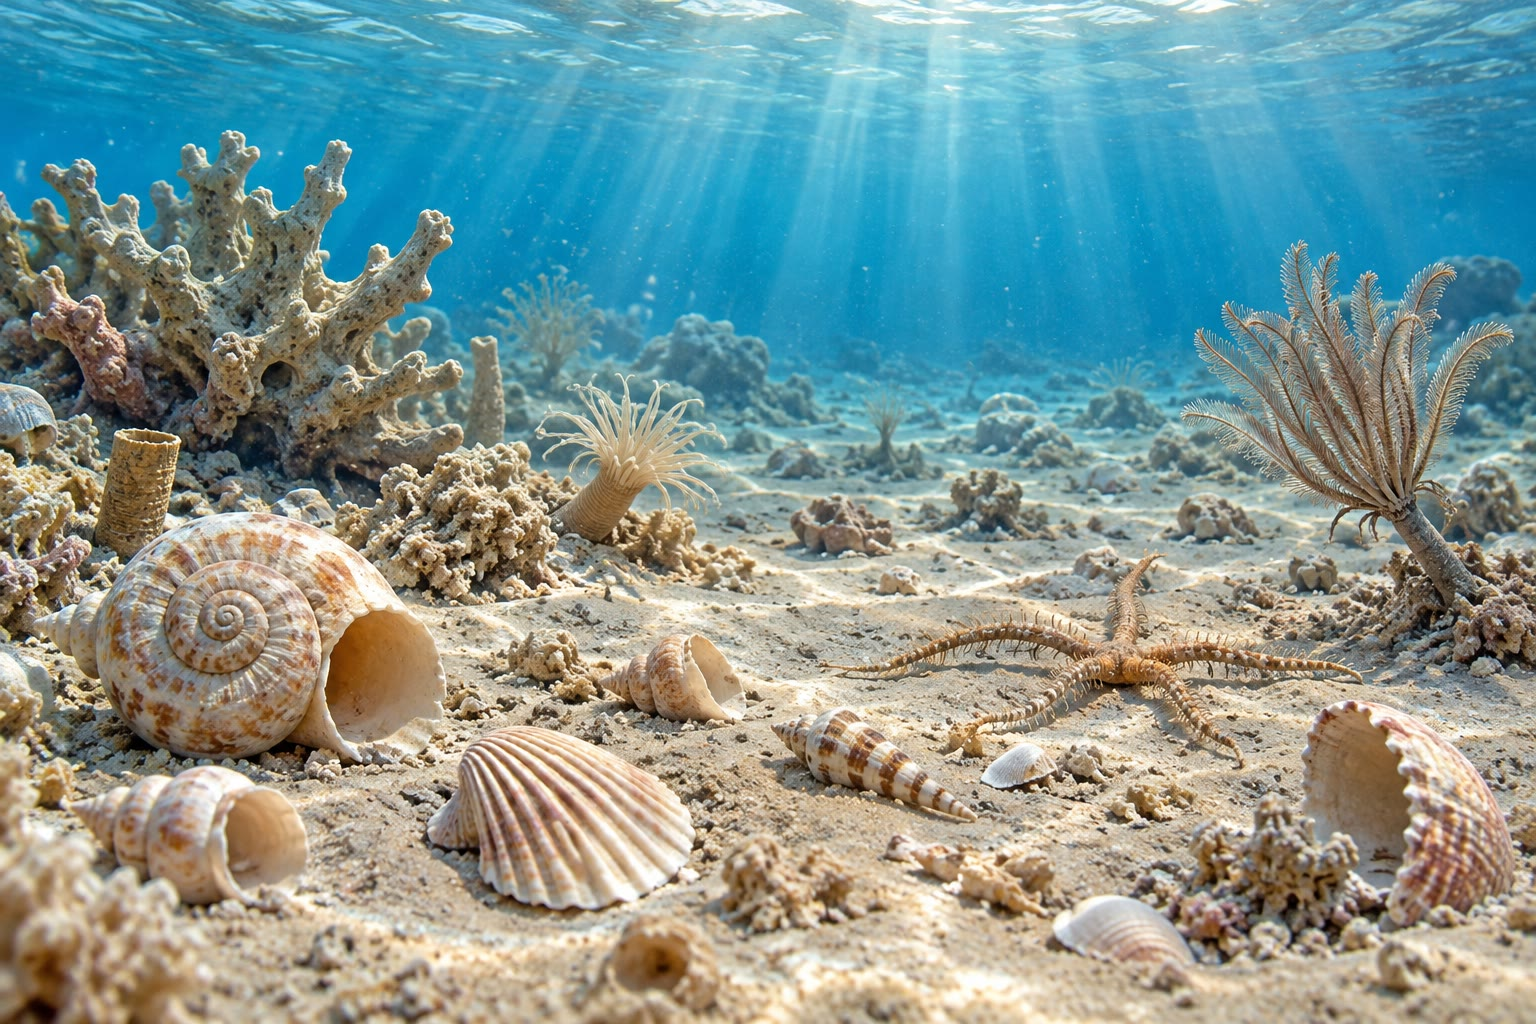
\includegraphics[width=0.6\linewidth]{images/book1/ai/g7-shallow-sea.jpg}

{\small Een warme, ondiepe zeebodem van lang geleden, zoals die eruit kan
hebben gezien terwijl schelpen en stukjes koraal neerdaalden in een
toekomstige kalksteen (door AI gegenereerde illustratie van een algemene
scène).}
\label{fig:g7:sediments-and-fossils:shallow-sea}
\end{omfigure}

\begin{remark}[Kijken, fotograferen, laten liggen]\label{rem:g7:sediments-and-fossils:leave}
Op veel beschermde plekken is het verboden een \omterm{def:g7:sediments-and-fossils:fossil}{fossiel} mee te nemen: in de
Grand Canyon is het bijvoorbeeld bij wet verboden om welk \omterm{def:g7:sediments-and-fossils:fossil}{fossiel} ook op te
graven, te verplaatsen of mee te nemen. Een bezoeker die er een vindt,
maakt een foto of een tekening, laat het liggen waar het ligt zodat anderen
het kunnen zien en wetenschappers het kunnen bestuderen, en waarschuwt een
boswachter.
\end{remark}
% ledger: nps:grca-fossils

\begin{inthefield}[Sedimenten die nu worden neergelegd]
Kijk op een strand, aan de oever van een \omterm{def:g1:landscapes-around-us:water}{meer} of langs een beek, samen met
een volwassene, naar het \omterm{def:g3:stones-pebbles-sand:sand}{zand} onder ondiep water: het stromende water vormt
er ribbels in, zoals die welke in het oude zandsteen bewaard zijn. Laat een
voetafdruk achter in het natte \omterm{def:g3:stones-pebbles-sand:sand}{zand} vlak bij de waterlijn en kijk wat de
volgende golven ermee doen. Kijk na een regenachtige dag naar een plas die
is opgedroogd: een dun laagje fijne modder bedekt vaak het \omterm{def:g3:stones-pebbles-sand:sand}{zand} op de
bodem --- de fijnste korrels bezonken het laatst, toen het water stilstond.
Teken wat je ziet, en noteer waar en wanneer.
\end{inthefield}
% ledger: nps:ripple-marks, ucmp:footprints, usgs:strata

\section{Oefeningen}

\begin{exercise}[$\star$]\label{exo:g7:sediments-and-fossils:1}
Koppel elk woord aan zijn betekenis: \omterm{def:g7:sediments-and-fossils:sediment}{sediment}; \omterm{def:g7:sediments-and-fossils:layer}{stratum}; \omterm{def:g7:sediments-and-fossils:fossil}{fossiel}; \omterm{def:g7:sediments-and-fossils:fossil}{afdruk};
\omterm{def:g7:sediments-and-fossils:fossil}{afgietsel}; \omterm{def:g7:sediments-and-fossils:fossil}{sporenfossiel}. (a) Een holte in een \omterm{def:g3:stones-pebbles-sand:rock}{gesteente} waar een schelp is
opgelost. (b) Een voetafdruk of een graafgang die in een \omterm{def:g3:stones-pebbles-sand:rock}{gesteente} bewaard
is. (c) Los materiaal dat door water, wind of ijs is neergelegd. (d) Een
stenen kopie die ontstaat als een holte zich met \omterm{def:g6:rocks-and-minerals:mineral}{mineralen} vult. (e) Een
plaat sediment die in één keer is neergelegd. (f) Het overblijfsel of
spoor van een levend wezen van lang geleden, bewaard in \omterm{def:g3:stones-pebbles-sand:rock}{gesteente}.
\end{exercise}

\begin{exercise}[$\star$]\label{exo:g7:sediments-and-fossils:2}
Zet deze stappen in de goede volgorde om te vertellen hoe een schelp een
\omterm{def:g7:sediments-and-fossils:fossil}{fossiel} aan het oppervlak wordt: (a) \omterm{def:g5:water-shapes-the-land:erosion}{erosie} slijt de lagen erboven weg;
(b) het dier sterft op de zeebodem; (c) nieuwe lagen stapelen zich op en de
schelp verandert in steen; (d) modder bedekt de schelp snel.
\end{exercise}

\begin{exercise}[$\star$]\label{exo:g7:sediments-and-fossils:3}
Gebruik de tabel met aanwijzingen. Waar is elke laag ontstaan? (a) Een
kalksteen vol koralen. (b) Een zandsteen met golfribbels op het oppervlak.
(c) Een donkere laag steenkool. (d) Een schalie met afdrukken van bladeren
en de vleugel van een libel.
\end{exercise}

\begin{exercise}[$\star$]\label{exo:g7:sediments-and-fossils:4}
Waar of niet waar? Verbeter de onware uitspraken. (a) Elk dier dat sterft,
wordt ooit een \omterm{def:g7:sediments-and-fossils:fossil}{fossiel}. (b) Een voetafdruk kan een \omterm{def:g7:sediments-and-fossils:fossil}{fossiel} zijn. (c) Als
modderig water vertraagt, bezinkt de fijne modder het eerst.
(d) \omterm{def:g7:sediments-and-fossils:sediment}{Sedimenten} worden vlak neergelegd.
\end{exercise}

\begin{exercise}[$\star\star$]\label{exo:g7:sediments-and-fossils:5}
Gebruik de kolom van de Varden Hills. (a) Geef de dikte van het zandsteen,
de kalksteen en de schalie. (b) Wat is hun totale dikte? (c) Welk
percentage van dit totaal is kalksteen? Rond af op een heel getal.
(d) Waarom geeft de kolom geen dikte voor het krijt?
\end{exercise}

\begin{exercise}[$\star\star$]\label{exo:g7:sediments-and-fossils:6}
Een leerling schudt een pot met water, \omterm{def:g3:stones-pebbles-sand:pebble}{grind}, \omterm{def:g3:stones-pebbles-sand:sand}{zand} en modder, en laat die
bezinken. (a) Teken de pot de volgende dag en benoem de lagen. (b) Waarom is
het water na een uur nog troebel? (c) Ze doet er weer \omterm{def:g3:stones-pebbles-sand:sand}{zand} en modder bij en
laat het bezinken. Wat ziet ze nu op de bodem? (d) Welke laag in de pot is
het eerst ontstaan?
\end{exercise}

\begin{exercise}[$\star\star$]\label{exo:g7:sediments-and-fossils:7}
Wat heeft de meeste kans om een \omterm{def:g7:sediments-and-fossils:fossil}{fossiel} te worden, en wat de minste? Leg
uit. (a) Een kwal die op een rotsige \omterm{def:g1:landscapes-around-us:water}{kust} is aangespoeld. (b) Een
slakkenhuis dat in de modder van een rustig meer is begraven. (c) Een bot
dat jarenlang op een droge \omterm{def:g1:landscapes-around-us:landform}{vlakte} ligt. (d) Een mosselschelp die bij een
\omterm{def:g5:water-shapes-the-land:flood}{overstroming} van een \omterm{def:g1:landscapes-around-us:water}{rivier} door \omterm{def:g3:stones-pebbles-sand:sand}{zand} wordt bedekt.
\end{exercise}

\begin{exercise}[$\star\star$]\label{exo:g7:sediments-and-fossils:8}
Een schelp is begraven in \omterm{def:g3:stones-pebbles-sand:sand}{zand} dat zandsteen wordt. Water dat door het
\omterm{def:g3:stones-pebbles-sand:rock}{gesteente} sijpelt, lost de schelp helemaal op. (a) Wat blijft er in het
\omterm{def:g3:stones-pebbles-sand:rock}{gesteente} over? (b) Later vullen \omterm{def:g6:rocks-and-minerals:mineral}{mineralen} deze holte op. Wat ontstaat er?
(c) Is de schelp zelf er nog? (d) Waarom worden afdrukken en \omterm{def:g7:sediments-and-fossils:fossil}{afgietsels}
vaker in zandsteen gevonden dan in schalie? (Denk na over hoe gemakkelijk
water tussen de korrels door gaat.)
\end{exercise}

\begin{exercise}[$\star\star$]\label{exo:g7:sediments-and-fossils:9}
De Grand Canyon is gemiddeld \qty{1.6}{km} diep. (a) Schrijf deze diepte
in meter. (b) Stel dat de wanden van de canyon bestonden uit lagen van elk
\qty{80}{m} dik: hoeveel lagen zouden er van de rand tot de bodem passen?
(c) Welk percentage van de diepte is een laag van \qty{160}{m}?
\end{exercise}

\begin{exercise}[$\star\star$]\label{exo:g7:sediments-and-fossils:10}
In een zandsteen worden voetafdrukken van dinosaurussen gevonden. (a)
Liepen de dinosaurussen op hard \omterm{def:g3:stones-pebbles-sand:rock}{gesteente}? Leg uit. (b) Waarom verdwijnen
de meeste voetafdrukken op een modderige \omterm{def:g1:landscapes-around-us:water}{kust}? (c) Wat moest er kort nadat
de dinosaurussen voorbij waren gekomen gebeuren om de voetafdrukken te
bewaren? (d) Is een voetafdruk een lichaamsfossiel of een \omterm{def:g7:sediments-and-fossils:fossil}{sporenfossiel}?
\end{exercise}

\begin{exercise}[$\star\star\star$]\label{exo:g7:sediments-and-fossils:11}
In een \omterm{def:g1:landscapes-around-us:water}{meer} laat elke \omterm{def:g5:water-shapes-the-land:flood}{overstroming} een laag \omterm{def:g3:stones-pebbles-sand:sand}{zand} van ongeveer \qty{2}{cm}
dik achter, en de rustige weken daarna een laag modder van ongeveer
\qty{5}{mm} dik (gegevens voor de oefening). (a) Hoe dik is één paar lagen,
in millimeter? (b) Een boorkern uit de bodem van het \omterm{def:g1:landscapes-around-us:water}{meer} is \qty{1}{m}
lang en bestaat alleen uit zulke paren. Hoeveel \omterm{def:g5:water-shapes-the-land:flood}{overstromingen} legt hij
vast? (c) Bij de riviermonding zijn de zandlagen dikker, ver weg zijn ze
dunner. Leg uit waarom. (d) Waarom is er ver van de \omterm{def:g5:water-shapes-the-land:source-mouth}{monding} meer modder dan
\omterm{def:g3:stones-pebbles-sand:sand}{zand}?
\end{exercise}

\begin{exercise}[$\star\star\star$]\label{exo:g7:sediments-and-fossils:12}
De \omterm{def:g7:sediments-and-fossils:fossil}{fossielen} die in \omterm{def:g3:stones-pebbles-sand:rock}{gesteenten} worden gevonden, zijn vooral schelpen en
piepkleine resten; \omterm{def:g7:sediments-and-fossils:fossil}{fossielen} van zachte dieren zijn zeldzaam, en
dinosaurussen vormen maar een heel klein deel van alle \omterm{def:g7:sediments-and-fossils:fossil}{fossielen}. (a) Leg
uit waarom schelpen zo algemeen zijn. (b) Leg uit waarom zachte dieren
zeldzaam zijn. (c) Een wetenschapper wil alle dieren kennen die in een
oude \omterm{def:g2:water-on-earth:ocean}{zee} leefden. Kunnen de \omterm{def:g7:sediments-and-fossils:fossil}{fossielen} de volledige lijst geven? Leg uit.
\end{exercise}

\section{Probleem: De kolom van de Varden Hills}

\begin{problem}[{Weekendprobleem --- de lagen van de Varden Hills worden een
voor een gelezen, hun fossielen vertellen waar ze ontstonden, en de tijd
die nodig was om de kalksteen op te stapelen wordt berekend}]
\label{pb:g7:sediments-and-fossils:1}
% ledger: (invented region: figdata/shared/region.py; rates are exercise data, figdata/grade-7/varden_column.py part rates)
Gebruik de kolom van de Varden Hills in dit hoofdstuk. Het zandsteen
vertoont golfribbels en voetafdrukken; de kalksteen bevat koralen en
schelpen; de schalie bestaat uit heel fijne korrels, met ammonieten; het
krijt bovenaan is gedeeltelijk weggesleten.

\medskip
\noindent\textbf{Deel I --- De lagen lezen.}\par\nopagebreak
\begin{enumerate}[beginpenalty=10000]
  \item Noem de vier lagen, van de eerste die werd neergelegd tot de
        laatste.
  \item Geef de dikte van het zandsteen, de kalksteen en de schalie, en hun
        totaal.
  \item Welk percentage van dit totaal is kalksteen?
  \item Waarom kan niemand zeggen hoe dik het krijt was toen het ontstond?
\end{enumerate}

\medskip
\noindent\textbf{Deel II --- De fossielen erin.}\par\nopagebreak
\begin{enumerate}[resume, beginpenalty=10000]
  \item Waar is het zandsteen ontstaan? Geef twee aanwijzingen.
  \item Waar is de kalksteen ontstaan? Geef de aanwijzing.
  \item De schalie bestaat uit heel fijne korrels. Was het water rustig of
        stromend toen ze werd neergelegd? Leg uit.
  \item Vertel in drie zinnen het verhaal van de plek, van het zandsteen
        tot de schalie.
\end{enumerate}

\medskip
\noindent\textbf{Deel III --- Hoe lang het duurde.}\par\nopagebreak
\begin{enumerate}[resume, beginpenalty=10000]
  \item Schrijf de dikte van de kalksteen in centimeter.
  \item Stel dat het zandsteen elke 20 jaar \qty{1}{cm} aangroeide. Hoeveel
        jaar duurden zijn \qty{120}{m}?
  \item Stel dat de kalksteen elke 100 jaar \qty{1}{cm} aangroeide. Hoeveel
        jaar duurde \qty{1}{m} kalksteen?
  \item Hoeveel jaar duurde de \qty{180}{m} kalksteen? Hoeveel keer langer
        is dat dan voor het zandsteen?
\end{enumerate}
\end{problem}
